% Shared TikZ scaffold for OpenResearch figures.
\documentclass[border=2pt]{standalone}
\usepackage{tikz}
\usepackage{amsmath}
\usetikzlibrary{arrows.meta, positioning, fit, backgrounds, calc, shapes.geometric}

\definecolor{orxblue}{HTML}{0072B2}
\definecolor{orxorange}{HTML}{E69F00}
\definecolor{orxgreen}{HTML}{009E73}
\definecolor{orxred}{HTML}{D55E00}
\definecolor{orxpurple}{HTML}{CC79A7}

\tikzset{
  orx/.style={
    font=\sffamily\footnotesize,
    >={Stealth[round, length=4pt, width=3pt]},
    line width=0.5pt,
    node distance=4.5mm and 8.5mm,
  },
  block/.style={
    draw=black!55, fill=white, rounded corners=1pt,
    minimum height=6.5mm, minimum width=17mm, inner sep=2.5pt, align=center,
  },
  ours/.style={block, draw=orxblue, fill=orxblue!7, line width=0.7pt},
  muted/.style={block, draw=black!30, fill=black!3, text=black!65},
  data/.style={
    draw=black!45, fill=black!2, trapezium,
    trapezium left angle=78, trapezium right angle=102,
    minimum height=6mm, inner sep=2pt, align=center,
  },
  stage/.style={
    draw=black!25, dashed, rounded corners=2pt, inner sep=3.5pt, fill=black!1,
  },
  stagelbl/.style={font=\sffamily\scriptsize, text=black!55},
  flow/.style={->, draw=black!70},
  backflow/.style={->, densely dashed, draw=orxred!85},
  edgelbl/.style={font=\sffamily\scriptsize, text=black!65, inner sep=1.2pt},
}

\begin{document}
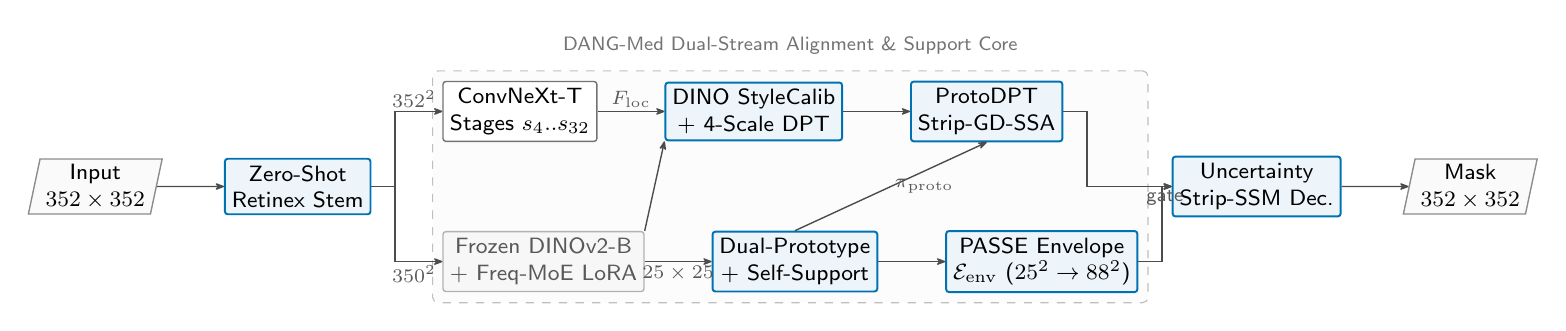
\begin{tikzpicture}[orx]

  \node[data] (input) {Input\\$352\times 352$};
  \node[ours, right=of input] (stem) {Zero-Shot\\Retinex Stem};

  \node[block, above right=2mm and 9mm of stem] (cnn) {ConvNeXt-T\\Stages $s_4..s_{32}$};
  \node[muted, below right=2mm and 9mm of stem] (vit) {Frozen DINOv2-B\\+ Freq-MoE LoRA};

  \node[ours, right=of cnn] (calib) {DINO StyleCalib\\+ 4-Scale DPT};
  \node[ours, right=of vit] (proto) {Dual-Prototype\\+ Self-Support};

  \node[ours, right=of calib] (gdssa) {ProtoDPT\\Strip-GD-SSA};
  \node[ours, right=of proto] (passe) {PASSE Envelope\\$\mathcal{E}_{\mathrm{env}}$ ($25^2\to 88^2$)};

  \node[ours, right=9mm of $(gdssa.east)!0.5!(passe.east)$] (dec) {Uncertainty\\Strip-SSM Dec.};
  \node[data, right=of dec] (out) {Mask\\$352\times 352$};

  \draw[flow] (input) -- (stem);
  \draw[flow] (stem.east) -- ++(3mm,0) |- node[edgelbl, pos=0.7, above] {$352^2$} (cnn.west);
  \draw[flow] (stem.east) -- ++(3mm,0) |- node[edgelbl, pos=0.7, below] {$350^2$} (vit.west);

  \draw[flow] (cnn) -- node[edgelbl, above] {$F_{\mathrm{loc}}$} (calib);
  \draw[flow] (vit) -- node[edgelbl, below] {$25\times 25$} (proto);
  \draw[flow] (vit.north east) -- (calib.south west);

  \draw[flow] (calib) -- (gdssa);
  \draw[flow] (proto.north) -- node[edgelbl, right] {$\pi_{\mathrm{proto}}$} (gdssa.south);
  \draw[flow] (proto) -- (passe);

  \draw[flow] (gdssa.east) -- ++(3mm,0) |- (dec.west);
  \draw[flow] (passe.east) -- ++(3mm,0) |- node[edgelbl, pos=0.65, below] {gate} (dec.west);
  \draw[flow] (dec) -- (out);

  \begin{scope}[on background layer]
    \node[stage, fit=(cnn)(vit)(calib)(proto)(gdssa)(passe)] (trunk) {};
  \end{scope}
  \node[stagelbl, above=0.8mm of trunk] {DANG-Med Dual-Stream Alignment \& Support Core};

\end{tikzpicture}
\end{document}
